\documentclass[12pt,italian]{report}
\usepackage{tesi}

\usepackage[a4paper]{geometry}		% Formato del foglio
\usepackage[italian]{babel}			% Supporto per l'italiano
\usepackage[utf8]{inputenc}			% Supporto per UTF-8
\usepackage[a-1b]{pdfx}				% File conforme allo standard PDF-A (obbligatorio per la consegna)

\usepackage{graphicx}				% Funzioni avanzate per le immagini
\usepackage{hologo}					% Bibtex logo with \hologo{BibTeX}
%\usepackage{epsfig}				% Permette immagini in EPS
%\usepackage{xcolor}				% Gestione avanzata dei colori
\usepackage{amssymb,amsmath,amsthm} % Simboli matematici
\usepackage{listings}				% Scrittura di codice
\usepackage{url}					% Visualizza e rendere interattii gli URL
\usepackage{hyperref}				% Rende interattivi i collegamenti interni

\def\myCDL{Corso di Laurea magistrale in\\Informatica}

% TITOLO TESI:
\def\myTitle{Sicurezza Hardware in Ambienti Virtualizzati Tramite un Passthrough TEE tra QEMU e Linux}

% AUTORE:
\def\myName{Marco Cutecchia}
\def\myMat{Matr. Nr. 983828}

% RELATORE E CORRELATORE:
\def\myRefereeA{Prof. Danilo Bruschi}

% ANNO ACCADEMICO
\def\myYY{2022-2023}

% Il seguente comando introduce un elenco delle figure dopo l'indice (facoltativo)
%\figurespagetrue

% Il seguente comando introduce un elenco delle tabelle dopo l'indice (facoltativo)
%\tablespagetrue

\begin{document}

\frontespizio
\afterpreface

% FIXME: Non compare sull'indice
\chapter*{Sommario}
\addcontentsline{toc}{chapter}{Sommario}  
\label{cap:sommario}
% + Chiediamo più servizi e dunque aumenta la superficie di attacco, ma un
%   buco anche in servizi non critici rischia di mettere a rischio l'intero
%   sistema
L'aumento dei servizi che vengono richiesti dai moderni dispositivi di
computazione ha creato un quesito: l'aspetto di sicurezza è diventato più
importante di prima, ma con la maggiore complessità di tali sistemi aumenta
anche la superficie di attacco.
Rimuovere funzionalità dal sistema principale per renderlo più sicuro non
è accettabile, ma è possibile isolare i servizi critici dal punto di vista
della sicurezza in ambienti di computazione separati.

Questa è l'idea alla base dei \textit{Trusted Execution Environment(TEE)},
creare un ambiente di computazione nel processore, isolato dal resto del
mondo non sicuro e dedicato solamente a quei software con requisiti di
sicurezza stringenti.

% + Molto diffusi su mobile, inizia ad esserci interesse su piattaforme cloud
%   (trusted computing)
Dato che gli smartphone stanno diventando sempre più critici per la nostra vita
i TEE sono estremamente diffusi in ambito mobile, dove la piattaforma ARM fa da
padrona, e ormai presenti su praticamente tutti i cellulari ma inizia a esserci
un crescente interesse al loro uso anche in ambito Desktop e, in particolare,
anche sui server grazie all'iniziativa \textit{Confidential Computing}.

% + Esistono soluzioni ma sono solo su piattaforme x86 via intel SGX che è una
%   implementazione molto particolare(approfondire)
% + Con il crescente interesse nell'uso di ARM sui server vogliamo scoprire
%   come integrare un TEE implementato via TrustZone in ambienti virtualizzati
Al momento di scrittura di questa tesi, il mercato server è principalmente
dominato da processori basati sull'architettura x86\_64, esiste però un
interesse nell'uso di processori basati su architettura ARM grazie alla loro
particolare efficienza energetica.
Lo scopo di questa tesi è studiare come è possibile rendere disponibili i
servizi offerti da un TEE conforme alla specifica GlobalPlatform anche ad
ambienti virtualizzati.

% + Implementato un prototipo tramite QEMU, Linux ed utilizzando OP-TEE come
%   test case di TEE
Il risultato è stato quello di una versione modificata dell'emulatore QEMU
per aggiungere un device virtuale per la comunicazione tra il guest e il TEE
disponibile all'host. Inoltre è stato sviluppato un driver per sistemi Linux
e testato su piattaforma ARM usando OP-TEE come TEE di prova.

% TODO: PARLA DI PROBLEMI

% Le soluzioni disponibili sul mercato fanno uso di Intel SGX
% o AMD SEV, che descriviamo rispettivamente in \ref{sec:intel-sgx} e
% \ref{sec:amd-sev}. Queste tecnologie sono disponibili solamente su processori
% con architettura x86\_64 dei rispettivi produttori hardware.
% Con un maggior interesse nell'utilizzo dell'architettura ARM lato server, % FIXME: Cit required
% grazie alla sua maggior efficienza energetica, % FIXME: Cit required
% vogliamo dunque trovare una soluzione equivalente per questa architettura.
% 
% Fino a oggi la gran parte degli sforzi rispetto all'uso dei TEE su ARM
% si è concentrata su dispositivi mobile, ma il modello dei TEE come implementato
% su questi dispositivi non può essere trasposto direttamente sui server,
% richiede di risolvere dei nuovi problemi nati dal diverso ambiente.
% In particolare i TEE dei dispositivi mobile sono pensati per essere usati
% da un solo utente, mentre in un ambiente cloud è necessario che più utenti
% possano usare la stessa macchina fisica e dunque che il TEE possa essere
% condiviso.
% Inoltre, il modello dei TEE mobile assume che il software rimanga legato a
% un unico TEE per tutta la sua esecuzione; questa assunzione cade in ambito
% cloud dato che una VM potrebbe essere trasferita su in qualunque momento su
% una macchina fisica diversa, e dunque su un TEE diverso.


\chapter{Introduzione}
\label{sec:introduzione}
I sistemi informatici moderni sono estremamente complessi e sono composti da
molti componenti diversi che interagiscono continuamente tra di loro.
Questa complessità può rendere difficile garantire che questi sistemi siano
sicuri e dunque privi di vulnerabilità.

Una delle ragioni è che il gran numero di componenti e le interazioni tra di
essi possono rendere difficile testare e verificare in modo completo la
sicurezza di un sistema.
Ad esempio, un sistema potrebbe contenere al suo interno un componente che
singolarmente non ha vulnerabilità ma che potrebbero aprire una falla di
sicurezza quando combinato con un altro.
Dato l'incredibile numero di combinazioni possibili, è molto difficile
prevedere e valutare accuratamente il rischio di vulnerabilità di un sistema
in anticipo, in modo da implementare contromisure efficaci.

Un'altra ragione è che i sistemi informatici sono in costante evoluzione, con
l'aggiunta di nuove funzionalità e capacità nel corso del tempo.
Ciò può rendere difficile mantenere la sicurezza di un sistema, poiché nuove
vulnerabilità potrebbero sorgere a causa di modifiche che all'apparenza non
avrebbero dovuto avere tale effetto.

In generale vale la regola che più un sistema è semplice, più è facile testare
e verificare la sua sicurezza.
Ridurre la complessità dei moderni sistemi è una idea nobile ma che si scontra
presto con la realtà: una moltitudine di fattori, sia tecnici sia economici,
rende difficile attuare questo piano senza dover scendere a compromessi.

\bigbreak \noindent

Una proposta alternativa e più realistica è quella data dai
\textit{Trusted Execution Environments} (TEE).
I TEE, come suggerisce il nome, sono ambienti sicuri in cui è possibile
eseguire del software. Date le caratteristiche dei TEE, dentro essi
generalmente si esegue solamente software con necessità di sicurezza
particolarmente stringenti.

L'idea di un TEE è quella di fornire all'interno del dispositivo
un secondo sistema isolato dall'altro; questo, essendo
indipendente, può implementare delle policy di sicurezza più
stringenti rispetto a quelle del sistema principale senza però dover
rinunciare a funzionalità.

Un TEE, come il sistema principale, contiene al suo interno un sistema
operativo e dei programmi scritti per esso, ma tramite l'uso di tecniche
crittografiche, hardware di supporto e un approccio di sviluppo che
prioritizza la sicurezza sopra tutti gli altri aspetti è possibile
offrire un grado di sicurezza molto più elevato rispetto a quello
offerto da un sistema tradizionale.

\bigbreak \noindent

Un calcolatore provvisto di TEE può essere visto come un sistema composto da
due calcolatori, dove uno di essi è dedicato solamente a garantire la sicurezza
del sistema nel suo complesso.
Questa non è una metafora: un TEE può essere implementato in diversi modi ma
uno di essi è quello di utilizzare un \textit{System on a Chip} che viene
inserito all'interno del processore principale.
Esempi di questo tipo di TEE sono la \textit{Secure Enclave}
di \textit{Apple} oppure il \textit{Platform Security Processor} presente
in molti processori \textit{AMD Ryzen}, che ironicamente al loro interno
includono un processore della concorrente \textit{ARM}.

Includere un secondo calcolatore all'interno del primo è un'idea efficace,
ma non è l'unico modo di implementare un TEE.
In generale però è possibile dire che per implementare un TEE è necessario
di supporto hardware dedicato, questo perché il software da solo non è in
grado di potersi difendere da altro software quando questo ha i suoi
stessi privilegi.

\section{Cloud computing e sicurezza}
\label{sec:cloud}
Gli ultimi anni hanno visto un cambiamento radicale nel modo in cui
i produttori di software possono distribuire i loro prodotti
grazie alla affermazione del \textit{Cloud Computing}.

In passato l'unico modo per offrire un servizio web era quello di
comprare o affittare dei server, dovendo occuparsi della loro manutenzione
e dovendo prevedere la capacità di questi in base alle previsioni di
utilizzo.
Con il modello \textit{cloud} nasce il concetto di
\textit{Infrastructure as a Service}, cioè la possibilità di affittare
l'intera infrastruttura di rete necessaria a eseguire la nostra applicazione
web e lasciare l'onere di mantenerla al provider cloud.

Il cloud computing è diventato estremamente popolare negli ultimi anni
grazie alla sua capacità di offrire risorse flessibili a basso costo
anche a piccole e medie imprese.
Questo modello è redditizio sia per i fornitori che per gli utenti,
con i fornitori che possono offrire servizi a un costo inferiore grazie
alle economie di scala e gli utenti che possono ridurre i costi IT e
aumentare la loro agilità e competitività.

\bigbreak \noindent

Ovviamente questo modello porta non solo vantaggi, ma anche nuove sfide
in termini di sicurezza.
L'uso di questo modello comporta che i dati e il codice vengano spostati
su server remoti che non sono più in mano nostra.
Il controllo di questi server permette ai provider di ottimizzare al meglio
l'uso delle risorse fisiche disponibili e di offrire servizi a prezzi molto
convenienti, ma d'altro canto questo comporta una perdita del controllo
di cosa avviene al software durante l'esecuzione nei server e di 
chi può accedere ai dati oltre a loro.

Seppur sia lecito aspettarsi che i provider di servizi cloud siano onesti
e non vadano a sabotare i propri clienti, questa potrebbe non essere
una garanzia sufficiente per tutti.

Il modello di cloud include però un secondo attaccante: gli altri clienti.
Il modo in cui i provider possono permettersi di offrire servizi di cloud
computing a prezzi convenienti è quello di condividere i server tra più
clienti; utilizzando delle macchine virtuali un server
può ospitare le applicazioni di più clienti allo stesso momento.

L'uso della \textit{virtualizzazione} permette ai provider di isolare
i clienti tra di loro, ridimensionare
dinamicamente le risorse computazionali a loro offerte e di trasferire
i loro dati e applicazioni da un server a un altro in qualsiasi
momento.
Tutto ciò avviene in modo completamente trasparente ai clienti, che hanno la
sensazione di utilizzare un server dedicato,
ma permette ai provider di ottimizzare al massimo l'utilizzo delle risorse
fisiche e di bilanciare il carico di lavoro tra i server.

\bigbreak \noindent

Il partizionamento di un server tra i vari clienti viene effettuato
utilizzando un \textit{hypervisor}, un software che presiede la creazione
e la gestione delle macchine virtuali su un server fisico.
Un hypervisor è in grado di vedere e modificare i dati in memoria di tutte
le macchine virtuali, per questo motivo è un bersaglio particolarmente
interessante per gli attaccanti.
Un attaccante che riesce ad eludere le protezioni di un hypervisor può
potenzialmente manomettere i dati di tutti i clienti che utilizzano quel
server.

Trattare tutte le possibili problematiche in termini di sicurezza del
cloud computing non è lo scopo di questa tesi.
Quanto descritto finora è solo una delle tante sfide che il cloud computing
porta con sé, ma è sicuramente una delle più importanti data la sua alta
posta in gioco.

\section{Motivazione della tesi}
\label{sec:motivazione}
I TEE nascono principalmente in ambito mobile proprio perché questi dispositivi
sono diventati una parte sempre più importante della nostra vita quotidiana,
di conseguenza sono diventati un bersaglio sempre più attraente per i
cybercriminali.
Oggi i TEE sono presenti su quasi tutti i cellulari, dove vengono usati per
eseguire operazioni sensibili come ad esempio le schermate di sblocco
del telefono e di inserimento di dati bancari o più in generale al
trattamento di chiavi crittografiche e dati sensibili;
il loro uso non è limitato però a questo ambito.

In particolare siamo interessati al loro utilizzo insieme al modello di
computing cloud per proteggere i dati.
Parlando di protezione dati nel cloud possiamo far riferimento a tre
aspetti:
\begin{itemize}
    \item \textbf{Dati in transito}: i dati devono essere protetti durante
    il trasferimento tra i client e i server.
    \item \textbf{Dati in storage}: i dati devono essere protetti anche
    quando sono inattivi sul server.
    \item \textbf{Dati in memoria}: i dati devono essere protetti durante
    l'esecuzione del codice sul server.
\end{itemize}

Se per i primi due aspetti esistono soluzioni ben consolidate, come ad
esempio il protocollo HTTPS per la protezione dei dati in transito e
l'uso di dischi cifrati per la protezione dei dati in archiviazione,
per l'ultimo aspetto non esiste ancora una soluzione standard.

Questo problema ha portato alla fondazione
della Confidential Computing Initiative (CCI), un gruppo di aziende che
si sono unite per sviluppare soluzioni per garantire la sicurezza dei dati
e del codice in ambito cloud computing mentre sono in memoria.

La CCI trova nei TEE un ottimo strumento per garantire la sicurezza dei dati
e del codice, ma il supporto oggi presente è limitato a server con
piattaforme Intel o AMD e con pesanti lock-in rispetto la piattaforma scelta.

Con un interesse crescente all'uso di architetture diverse da \texttt{x86\_64}
in ambito server, diventa sensata l'idea di sviluppare un sistema per
permettere l'utilizzo dei TEE in modo agnostico alla piattaforma sottostante.

\bigbreak \noindent

Lo scopo di questa tesi è dunque il primo passo verso questo obiettivo,
cioè sviluppare un canale di comunicazione tra una macchina virtuale e
un generico TEE, in modo completamente agnostico alla piattaforma
hardware sottostante e al codice in esecuzione dentro al TEE.

Il software sviluppato in questa tesi non vuole essere un prodotto finito,
ma un prototipo che dimostri la fattibilità del progetto e che permetta
di iniziare a discutere di come implementare un sistema completo.
A tale scopo abbiamo deciso di estendere l'hypervisor QEMU e il sistema
operativo Linux per permettere la comunicazione tra una macchina virtuale
gestita dal primo e un TEE collegato al secondo.

\section{Struttura della tesi}
\label{sec:struttura-tesi}
La tesi è strutturata in quattro capitoli principali:
\begin{itemize}
    \item Nel \textbf{Capitolo \ref{chap:tee}} diamo una introduzione al
    concetto di Trusted Execution Environment, alle sua applicazioni
    e a vari concetti correlati.
    \item Nel \textbf{Capitolo \ref{chap:hardware-supporto-tee}} discutiamo
    brevemente di varie soluzioni hardware a supporto dei TEE, delle loro
    caratteristiche e delle loro limitazioni.
    \item Nel \textbf{Capitolo \ref{chap:passthrough-tee-qemu-linux}}
    finalmente discutiamo del progetto di questa tesi, ovvero la creazione
    di un canale di comunicazione tra una macchina virtuale e un TEE.
    \item Infine nel \textbf{Capitolo \ref{chap:testing}} descriviamo
    come abbiamo testato il nostro prototipo e quali sono i risultati
    ottenuti.
\end{itemize}

In aggiunta a questi capitoli troviamo due appendici \ref{app:faketee} e
\ref{app:impostazione-ambiente-sviluppo-testing} che, seppur non essenziali
per la comprensione della tesi,
possono essere utili per risolvere alcune questioni tecniche
nel caso si fosse interessati a riprodurre o continuare il nostro lavoro.

\chapter{Trusted Execution Environment}
\label{chap:tee}
Un \textit{Trusted Execution Environment} (TEE) è un'area protetta in un
dispositivo che può essere utilizzata per eseguire codice autenticato in modo
più sicuro e attendibile rispetto al resto del sistema.

I TEE stanno diventando sempre più importanti man mano che i dispositivi
diventano più connessi e vulnerabili agli attacchi.
Forniscono un modo per proteggere i dati e le operazioni sensibili
dall'accesso o dalla modifica da parte di parti non autorizzate e possono
essere utilizzati per rendere possibili una vasta gamma di applicazioni
in molti ambiti, di cui parliamo in \ref{sec:applicazioni-tee}.

Data l'importanza che i dispositivi mobile stanno assumendo nella nostra
vita di tutti i giorni non dovrebbe sorprendere il fatto che i TEE sono
presenti su praticamente tutti i cellulari, grazie anche agli sforzi
pionieristici di ARM con la loro piattaforma \textit{TrustZone}.
Gli esempi di TEE in questo ambito sono numerosi, alcuni nomi noti sono
Samsung Knox, Qualcomm QSEE, Google Titan-M e Apple Secure Enclave.

L'utilizzo dei TEE non è assolutamente prerogativa solo del mondo mobile.
L'interesse verso i TEE sta crescendo anche in ambito IoT, Desktop e Server 
dove iniziamo a vedere sul mercato le prime soluzioni che permettono di
eseguire software in un ambiente protetto anche su queste piattaforme.

In questo capitolo illustriamo le caratteristiche chiave dei TEE e come
possono essere utilizzati per migliorare la sicurezza e l'affidabilità di
vari tipi di dispositivi e sistemi.

\section{TEE conformi GlobalPlatform}
\label{sec:tee-conformi-globalplatform}
I Trusted Execution Environment sono la combinazione di hardware e software
dedicato allo scopo di creare un ambiente di computazione protetto e sicuro.
Nonostante questa definizione, il termine "TEE" è piuttosto generico
e viene applicato a una vasta gamma di prodotti che hanno garanzie di sicurezza
e dettagli d'implementazione significativamente diversi.

La mancanza di una definizione comune e standardizzata dei TEE non solo rischia
di confondere i consumatori, ma può anche essere un ostacolo per gli sviluppatori
interessati a creare applicazioni che possono essere eseguite su più TEE
dato che devono gestire una vasta gamma di differenze in termini di come i
TEE sono implementati e quali garanzie di sicurezza effettivamente offrono.

Allo scopo proprio di risolvere questi problemi, nel 2010 il consorzio
GlobalPlatform ha pubblicato la prima versione dei documenti di specifica
per i TEE, oggi arrivati alla versione 1.3 pubblicati nel 2020.
Questi standard definiscono un set comune di guide linea e requisiti per la
creazione di TEE progettati per essere interoperabili e sicuri.

Più nel dettaglio, tra queste specifiche troviamo una architettura
generica per i TEE, un profilo di sicurezza e delle interfacce per
programmatori che permettono lo sviluppo di applicazioni portabili tra TEE
diversi. 

Diverse aziende e organizzazioni hanno adottato questi standard
ed hanno adattato le loro soluzioni per essere conformi alla specifica
GlobalPlatform.
Seppur esistano ancora sul mercato soluzioni non conformi non è difficile
prevedere che nel breve futuro la maggior parte dei TEE lo saranno.

Per questo motivo e altri motivi la discussione in questa tesi sarà limitata
ai TEE conformi GlobalPlatform.

\subsection{Architettura TEE}
\label{subsec:architettura-tee}

La specifica GlobalPlatform non detta una architettura per i TEE ma offre
comunque degli esempi che possono essere utili a comprendere quali sono
i componenti fondamentali di un TEE GlobalPlatform e come collaborano
tra di loro per l'implementazione.

% FIXME: Considera tradurre il testo in questa figura
% GPT TEE PP => Protection Profile
\begin{figure}
    \centering
    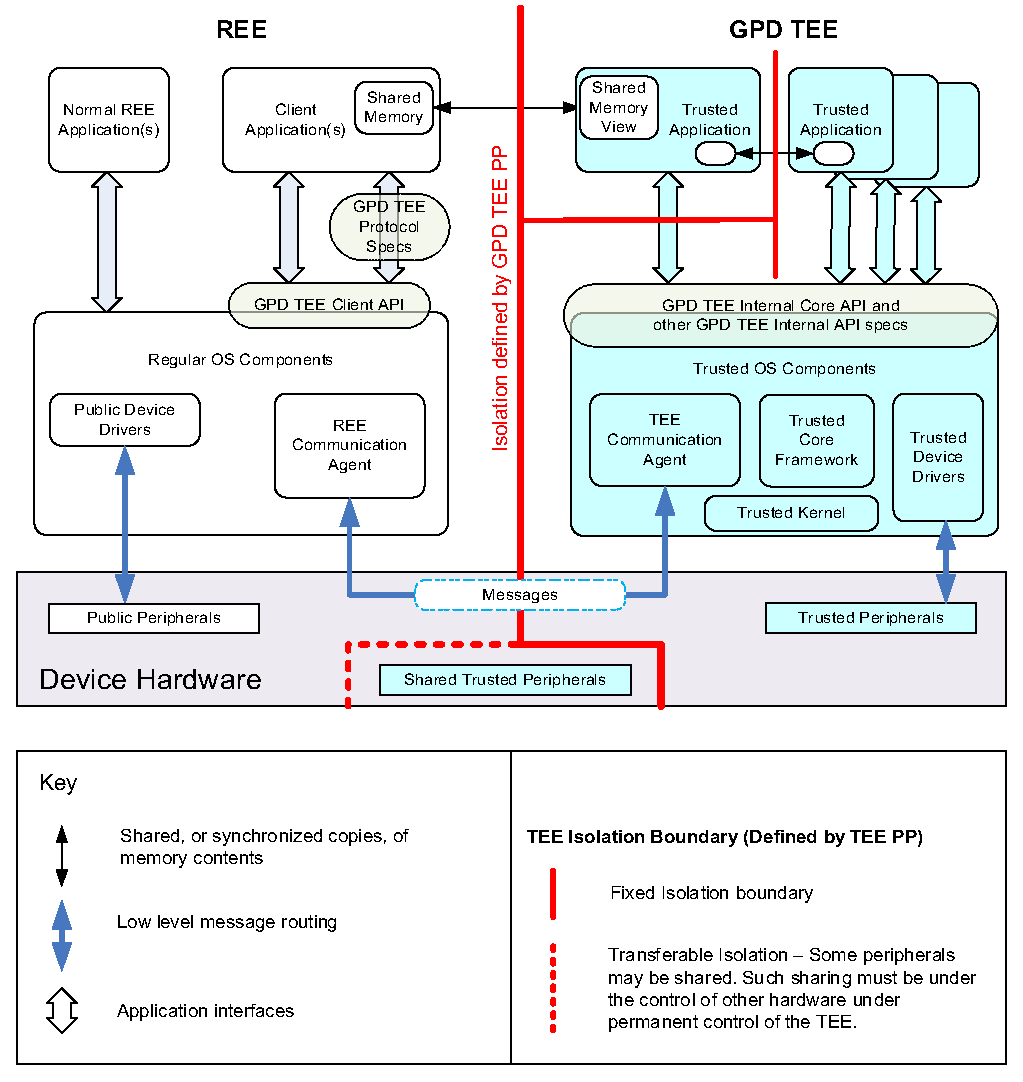
\includegraphics[width=1\textwidth]{immagini/tee-system-architecture}
    \caption{
        Architettura di un TEE conforme GlobalPlatform. 
        Da \textit{TEE System Architecture v1.3 (pag. 28)}
        \cite{gp2020systemarchitecture}
    }
    \label{fig:tee-system-architecture}
\end{figure}

In \figurename~\ref{fig:tee-system-architecture} è illustrata una possibile
architettura software di un sistema con un singolo TEE conforme
GlobalPlatform. Questa è solo una delle tante possibili architetture, inoltre
nulla vieta che un sistema possa avere più TEE, seppur nella pratica
questo non è molto comune.

In tale figura è possibile notare una barriera che divide il sistema in due
mondi: il mondo del \textit{Trusted Execution Environment} (TEE) a destra
e il mondo del \textit{Regular Execution Environment} (REE) a sinistra, cioè
il mondo a cui siamo abituati a lavorare con i sistemi operativi classici.

In entrambi i mondi troviamo un sistema operativo che gestisce le risorse
hardware e schedula l'esecuzione di processi. Un programma in esecuzione
dentro il TEE prende il nome di \textit{Trusted Application}(TA) e può
offrire dei servizi ad altre TA oppure alle applicazioni in esecuzione nel REE,
che prendono il nome di \textit{Client Application}(CA).

Le TA all'interno del TEE possono far uso del \textit{Trusted Core Framework}
che fornisce una interfaccia per operazioni comuni come il salvataggio
di file in modo sicuro, l'accesso al timer e altre funzionalità descritte
nella
\textit{Trusted Core Framework API Specification}\cite{gp2020internalapi}.
Questa interfaccia dovrebbe permettere di poter portare una TA su TEE diversi
senza doverne modificare il codice.

I due mondi non possono accedere direttamente all'altro, ma possono
comunicare solo tramite uno scambio di messaggi mediato dall'hardware.
Su questo meccanismo di comunicazione è possibile costruire meccanismi di
comunicazione a livello più alto, come ad esempio la condivisione di buffer
di memoria tra CA e TA.

\bigbreak \noindent

Il flusso di esecuzione solito è il seguente: una CA richiede un servizio a
una TA, per fare ciò utilizza la \textit{Client API} che astrae l'invio di un
messaggio al \textit{TEE Communication Agent}.
Questo primo messaggio apre una \textit{sessione} tra la CA e la TA, che
indica l'inizio di uno o più \textit{Function Invocation}.
Un messaggio di \textit{Function Invocation} contiene semplicemente un ID
che identifica la funzione da invocare e degli eventuali parametri;
il mapping tra ID e funzione è definito dalla \textit{Trusted Application}.
La TA esegue la funzione richiesta e risponde con un messaggio che contiene
l'esito dell'operazione ed eventuali dati di ritorno.

Queste chiamate sono sincrone, ma è possibile costruire delle chiamate
asincrone tramite un meccanismo di polling.

In entrambi i mondi troviamo dei \textit{Communication Agent}: questi 
hanno il compito d'inoltrare i messaggi tra CA e TA e, solo per il
\textit{TEE Communication Agent}, anche tra TA a TA.
I \textit{Communication Agent} possono prendere diverse forme nella pratica:
possono essere processi, componenti del sistema operativo ma anche semplici
librerie che vengono linkate alle applicazioni.
Seppur nello schema siano visti come solo due componenti, nella realtà il loro
ruolo può essere svolto usando più sotto-componenti.

\bigbreak

\noindent Infine, le periferiche hardware vengono suddivise in tre categorie:
\begin{itemize}
    \item \textit{Periferiche Fidate}: L'accesso a queste periferiche è
    consentito solamente dal TEE. Esempi di queste periferiche sono i
    sensori biometrici oppure memorie segrete % FIXME: Sensori biometrici? Memorie segrete? non ne sono sicuro 
    \item \textit{Periferiche Fidate Condivise}: L'accesso a queste
    periferiche di default è consentito solamente dal TEE, ma questo può
    decidere temporaneamente di condividere l'accesso con il REE. Esempi di
    queste periferiche sono il display e la tastiera.
    \item \textit{Periferiche Pubbliche}: L'accesso diretto a queste
    periferiche avviene dal REE, ma nulla impedisce a quest'ultimo di
    permettere l'accesso anche al TEE tramite un driver. Esempi di queste
    periferiche sono gli altoparlanti.
\end{itemize}

\subsection{Garanzie di sicurezza}
\label{subsec:garanzie-sicurezza}
I Trusted Execution Environment possono essere implementati in maniera
diversa tra di loro, di conseguenza non sarebbe corretto considerarli tutti
uguali dal punto di vista della sicurezza.
Per questo motivo, GlobalPlatform ha definito un set di proprietà che
devono essere garantite da tutti i TEE, queste sono elencate nel
\textit{Protection Profile}\cite{gp2020protectionprofile}.
Un TEE per essere certificato deve garantire almeno queste proprietà, ma
può garantire anche proprietà aggiuntive; questo vuol dire che rimane
comunque sensata l'osservazione che non tutti i TEE sono uguali, seppur
adesso sia possibile almeno stabilire una baseline minima. 

Una analisi dettagliata di questi documenti è fuori dallo scopo di questa
tesi, ma in generale è possibile affermare che un TEE deve poter garantire
la proprietà di esecuzione isolata rispetto al REE e le proprietà d'integrità
e confidenzialità sia del codice sia degli assets generati da esso.

Le specifiche GlobalPlatform non restringono come queste proprietà devono
essere raggiunte, seppur proponga alcune soluzioni pratiche.
Nonostante ciò esistono comunque degli aspetti comuni alla maggior parte dei
TEE, come ad esempio l'uso di supporto hardware per realizzare l'isolamento
oppure l'uso di firme digitali per garantire l'autenticità del codice.

% FIXME: Sarebbe interessante una sotto-sezione "Cosa non garantiscono i TEE"
%        (side-channel, attacchi di tipo hardware, ecc)

\paragraph{Isolamento:}
% TODO: Leggi per davvero l'articolo di rushby
Per garantire la proprietà d'isolamento dal REE, \cite{sabt2015tee} nota
che tutti i TEE implementano un \textit{separation kernel}
\cite{rushby1981separationkernel}. 
Un \textit{separation kernel} è un componente hardware e/o software fidato che
ha il compito di separare il sistema in zone isolate che non possono
interferire tra di loro e di mediare le comunicazioni tra di esse.
% FIXME: Sembra tanto l'idea di microkernel, bisogna approfondire la differenza
L'idea non è nuova, infatti venne proposta da Rushby nel 1981 dove propose
di vedere ogni singola macchina come un sistema distribuito di componenti
indipendenti, in questo modo un errore in un singolo componente non avrebbe
compromesso l'intero sistema.

Questa idea viene ripresa nel mondo dei TEE allo scopo di ridurre la
potenziale superficie di attacco del sistema, in questo modo se un
attaccante riesce a compromettere un singolo componente gli altri rimangono
intatti, assumendo che il \textit{separation kernel} non venga anch'esso
compromesso.

Nei sistemi operativi oggi in uso, come Linux o Windows, la superficie di
attacco è molto vasta a causa dell'enorme quantità di hardware che devono
supportare e il numero elevato di servizi, anche non critici per la sicurezza,
che offrono ai programmi utente. 
% FIXME: Qualche dato sulla dimensione di Linux/Windows? 
% Dati sugli exploit in quali parte del sistema(driver)?
Un attaccante che riesce a penetrare nel kernel ottiene il massimo livello di
controllo sulla macchina, diventa dunque sensata l'idea di separare quei
servizi importanti per la sicurezza e d'isolarli dal resto del sistema in
un ambiente sicuro.

Per questo motivo è importante che il \textit{separation kernel} sia
il più semplice possibile, in modo che sia verificabile facilmente che non
contenga falle di sicurezza.
Seppur sia possibile avere molteplici TEE sullo stesso sistema, nella pratica
tutte le implementazioni si limitano a un singolo TEE, dunque il
"sistema distribuito" immaginato da Rushby è composto solamente da due
componenti, il TEE e il REE.

% FIXME: Aggiungi e describi brevemente meglio esempi
% Esempi pratici di \textit{separation kernel} sono ARM TrustZone e
% Trusted Firmware-A, blablabla.

\paragraph{Integrità e autenticità:}
I benefici ottenibili tramite l'isolazione del TEE vengono annullati se
l'integrità e l'autenticità del codice e assets all'interno del TEE non
vengono garantite. Se così non fosse, un attaccante potrebbe modificare
il codice del TEE mentre il dispositivo è spento per poi riaccenderlo con
il codice compromesso.

Queste proprietà devono essere garantite nell'intero ciclo di vita del
sistema, non è accettabile che esse non vengano assicurate fin dal primo boot,
o che queste proprietà vengano temporaneamente non garantite, pena
l'impossibilità di poter dichiarare il sistema come non compromesso.

Una soluzione per assicurare l'integrità e autenticità del codice consiste
nell'implementare un meccanismo di autenticazione usando delle chiavi
private conosciute solamente da enti fidati.
Ogni software, prima di poter essere caricato dentro il TEE, dovrà prima
passare un processo di autenticazione che consiste nel confrontare un hash
calcolato sul codice con un hash firmato incluso con il software.
Questo hash deve essere firmato utilizzando una chiave privata riconosciuta
dal TEE, in questo modo esso può verificare che un ente fidato ha approvato
l'esecuzione del codice.

Unica eccezione a questa regola è il primissimo software mandato in esecuzione
sul sistema; questo non può essere autenticato perché non è ancora presente
alcun software in esecuzione che possa effettuare il processo di verifica.
Per ovviare al problema, questo software viene caricato da una memoria
impossibile da sovrascrivere, come ad esempio le PROM, in questo modo è
possibile assumere comunque che il software non sia stato compromesso.

\begin{figure}
\centering
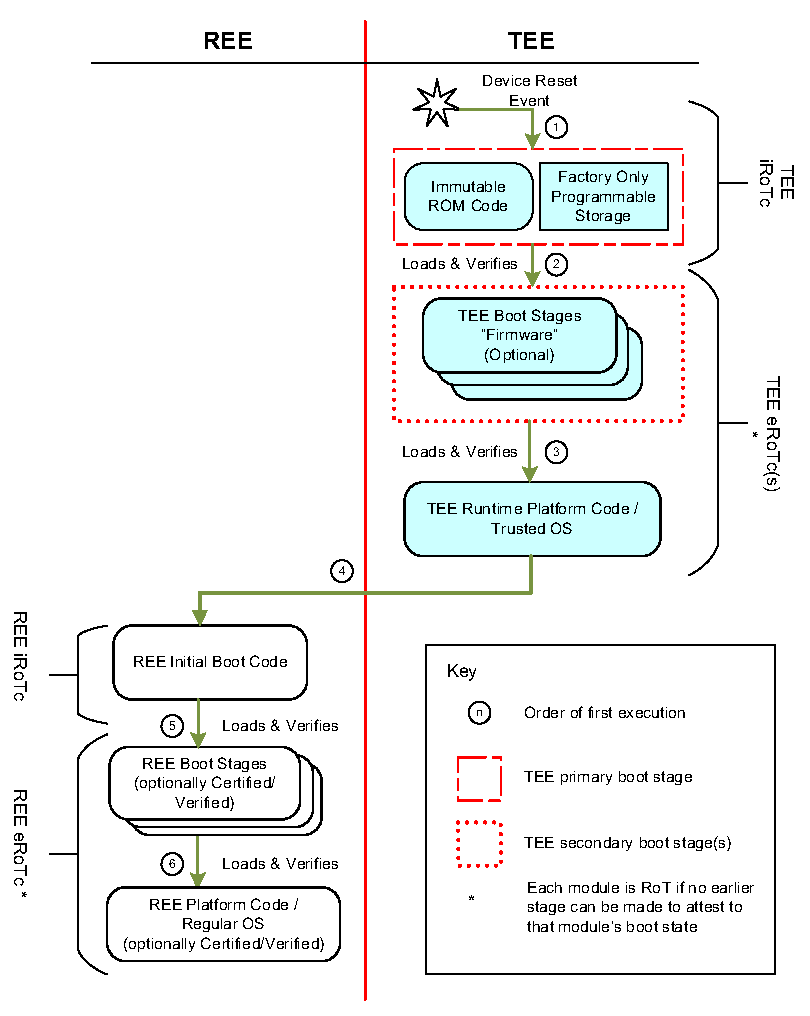
\includegraphics[width=0.8\textwidth]{immagini/tee-boot-sequence}
\caption{
    Sequenza di boot sicuro in un sistema con TEE. 
    Da \textit{GlobalPlatform TEE System Architecture pag. 73}
    \cite{gp2020systemarchitecture}
}
\end{figure}

Questo meccanismo di autenticazione è molto simile a quello utilizzato per
implementare il \textit{Secure Boot}; la differenza con quest ultimo è che
nel \textit{Secure Boot} la catena di verifica del software termina con
l'avvio del sistema operativo, questo perché \textit{Secure Boot} si prefigge
di autenticare solamente processo di avvio del sistema operativo.
In un TEE, invece, si spinge più in avanti e si verificano anche i programmi
eseguiti al suo interno.

In entrambi i casi, però, è necessario che il firmware di un dispositivo
conosca le chiavi pubbliche per poter verificare la firma dei software
da caricare. Come queste chiavi vengano ottenute dal firmware è un dettaglio
implementativo, dunque altamente dipendente dal sistema.

Per esempio, su PC che implementano \textit{UEFI Secure Boot} queste chiavi
vengono spesse memorizzate su una piccola memoria inclusa nella scheda madre % FIXME: Cit. required
oppure dentro un \textit{Trusted Platform Module}, % FIXME: Cit. required (si usano i TPM per questo scopo?)
un piccolo chip dedicato a operazioni crittografiche.

% FIXME: È un po' strano chiudere qui parlando di secure boot invece di TEE

\section{Applicazioni dei TEE}
\label{sec:applicazioni-tee}
I Trusted Execution Environment, con le loro maggiori garanzie d'integrità
e confidenzialità, non solo vengono utilizzati per aumentare la sicurezza
di applicazioni già esistenti, ma permettono lo sviluppo di nuove
applicazioni che non sarebbero possibili senza di essi.

Oggi i TEE sono largamente diffusi in ambito mobile, seppur non sempre
pubblicizzati, ma il loro utilizzo non è assolutamente limitato a tale ambito.
Le loro applicazioni sono molteplici ma sfortunatamente la grande
maggioranza dei produttori di dispositivi non supportano
l'installazione di software aggiuntivo dentro il TEE dopo la
configurazione iniziale.

Questo però potrebbe cambiare nei prossimi anni: proposte come
\cite{kohlbrenner2020opentees} o \cite{penglai} aprono a più sviluppatori la
possibilità di implementare i propri TEE.
Inoltre, a seguito dell'adozione da più vendor degli standard GlobalPlatform,
e lo sviluppo di TEE open-source come OP-TEE, potremmo vedere nei prossimi
anni un uso più ampio di questa tecnologia e aperto a tutti.

\subsection{Secure Storage}
\label{subsec:secure-storage}
Una delle feature più comuni è l'uso dei TEE per la creazione del
\textit{Secure Storage}, una zona di memoria non volatile che possa rimanere
al sicuro anche quando il dispositivo è spento.

Questa area viene crittografata utilizzando una chiave conosciuta solamente
all'interno del TEE, la decifratura dei dati avviene solamente a seguito di
un controllo degli accessi da parte del TEE.

Un utilizzo molto comune di questa area sicura è il salvataggio di dati
come l'impronta digitale degli utenti, dati di accesso a servizi online
oppure la gestione delle chiavi crittografiche.
Molti sviluppatori di applicazioni mobile Android e iOS utilizzano
quest'ultima funzionalità grazie ad API che, se presenti, utilizzano delle
TA, come ad esempio "Keystore"\cite{androidkeystore} in Android.

Alcuni produttori, ad esempio AMD con il suo
\textit{Platform Security Processor}, utilizzano la
funzionalità di \textit{Secure Storage} per implementare un
\textit{Trusted Platform Module}(TPM) software\cite{amd2020ftpm}.
Questo è normalmente un chip dedicato al salvataggio sicuro di chiavi crittografiche
ed allo svolgimento di varie operazioni di crittografia; re-implementando
queste operazioni dentro un TEE è dunque possibile per i produttori risparmiare
il costo dell'hardware normalmente necessario per un chip TPM.

Il \textit{Secure Storage} viene utilizzato non solo per salvare
informazioni di cui vogliamo mantenere la confidenzialità ma anche per
informazioni per cui vogliamo assicurarci che un attaccante non possa
modificare a suo piacere.
Un esempio di quest ultimo caso è il numero i tentativi fatti per sbloccare
un telefono: questa non è una informazione privata, ma non vogliamo che un
attaccante possa modificare questo valore per darsi più tentativi ed evitare
che il dispositivo si blocchi.

% FIXME: È comunque vulnerabile a rollback attack

\subsection{Remote Attestation}
\label{subsec:remote-attestation}
Uno degli usi possibili dei TEE è quello di fornire un meccanismo di
\textit{Remote Attestation} (RA), ovvero la possibilità di verificare che
un dispositivo remoto stia effettivamente eseguendo il software che
ci aspettiamo.

Il problema dell'attestazione remota è stato ben studiato negli anni e
sono stati proposti diversi metodi per risolverlo con vari gradi di
sicurezza.
La sfida principale è quella d'impedire a un attaccante di falsificare
i risultati dell'attestazione, ovvero di far credere a un altro dispositivo
che il dispositivo remoto stia eseguendo un software che non sta veramente
eseguendo.

In questo ambito i TEE possono essere utilizzati per implementare un sistema
di attestazione remota in modo molto semplice.
Un TEE, dato che offre integrità del software al suo interno, può implementare
una piccola \textit{Trusted Application} che ha il compito di eseguire
i controlli di attestazione e generare un report firmato digitalmente.
La chiave privata utilizzata per firmare il report può essere generata al
momento della prima installazione del dispositivo, questa chiave non uscirà
mai dal TEE, garantendo dunque la sicurezza.

Il tipico caso d'uso della RA è quello di una rete aziendale dove si
vuole verificare che nessun computer sia stato manomesso
e che non stiano eseguendo software non autorizzato.
Migliorare la sicurezza di sistemi già esistenti non è il suo unico utilizzo:
la RA può diventare un elemento fondamentale per lo sviluppo di nuove
applicazioni innovative, come discuteremo più avanti in questo capitolo.

\subsection{Protezione dei diritti di autore}
\label{subsec:drm}
Con la diffusione dei servizi di streaming, i produttori di contenuti esitano
a mettere a disposizione dei loro contenuti perché temono che questi vengano
condivisi con utenti che non hanno pagato per accedervi.
Effettivamente sarebbe molto semplice per un utente utilizzare un software per
registrare il proprio schermo mentre guarda un film acquistato legalmente, per
poi condividerlo con altri utenti senza che questi debbano acquistarlo.

Una applicazione molto diffusa dei TEE è il loro utilizzo per la protezione
dei diritti di autore (DRM). 
Sistemi come Widevine\cite{widevine} e PlayReady\cite{playready} vengono
integrati dai distributori di contenuti digitali allo scopo di impedire, o
almeno ostacolare, l'estrazione dei contenuti e la loro condivisione.
Questi sistemi hanno diversi livelli di protezione dei contenuti in base alle
capacità hardware del dispositivo; i produttori di contenuti possono richiedere
che un dispositivo supporti almeno un certo livello di sicurezza prima di
concedergli l'accesso ai propri contenuti.
Per esempio, alcuni servizi di streaming basati su Widevine richiedono che il
dispositivo raggiunga il livello L1 per poter usufruire di contenuti in alta
definizione; questo livello è raggiungibile solamente se presente un TEE con
la TA Widevine installata.

Il livello più alto di protezione che questi sistemi offrono è basato sui TEE,
che vengono usati per molteplici scopi tra cui: il provisioning di una chiave
crittografica condivisa tra server e client, la verifica delle licenze digitali
online e offline, la decrittazione degli stream audio/video e per mostrare
a schermo il video senza però che applicazioni esterne al TEE possano leggerne
i contenuti.
Per quest'ultima feature è necessario che sia presente un canale di
comunicazione fidato tra TEE e display, cioè che non dipenda dal REE, in modo
che un attaccante non possa leggere i pixel in chiaro che verranno mostrati poi
sullo schermo.

\subsection{Protezione dati nel Cloud}
\label{subsec:protezione-dati-cloud}
Il modello di computing cloud permette di sfruttare le risorse di calcolo
disponibili in maniera efficiente e scalabile, ma allo stesso tempo introduce
nuovi problemi di sicurezza.
Questo modello richiede di permettere al cloud provider di controllare la
nostra macchina per poterla gestire e monitorare; se da un lato questo solleva
gli sviluppatori dal dover occuparsi di gestire le macchine, dall'altro ciò
comporta un rischio di sicurezza.
Infatti, se il cloud provider è in grado di controllare la nostra macchina,
questo significa che può anche leggere i dati in memoria, che sono al sicuro
solo quando la macchina è spenta o in transito.

La situazione diventa ancora più problematica quando consideriamo che su
una singola macchina fisica i provider eseguono più macchine virtuali, ciascuna
di clienti diversi ma che condividono la stessa memoria fisica.
Ci sono stati molti esempi in passato di attaccanti che sono riusciti a eludere
le misure di sicurezza per isolare la propria VM dalle altre
\cite{vmescape1}\cite{vmescape2}\cite{vmescape3}.
Questi attaccanti avrebbero avuto la possibilità non solo di spiare le altre
VM dei clienti che hanno avuto la sfortuna di risiedere sullo stesso server in
quel momento, ma anche di manipolare il loro codice per i loro scopi.

Una organizzazione che dipende dal cloud e con particolari requisiti in
termini di sicurezza potrebbe dunque volere una sorta di garanzia che il
software che sta eseguendo sia quello che è stato consegnato al provider.
Questo è il problema della attestazione remota, per cui abbiamo già discusso
in \ref{subsec:remote-attestation} come i TEE possono aiutare.

La Confidential Computing Initiative\cite{confidential_computing_initiative}
è un consorzio di grandi aziende nel mondo cloud che lavora a questo problema
e che, al momento, trova nei TEE il modo per risolverlo.
Lo scopo dell'organizzazione è proprio quello di supportare lo sviluppo
di strumenti open source per garantire la s icurezza dei dati in memoria.
Questo è un campo di ricerca molto attivo e con molti progetti in corso ma
ancora poche soluzioni concrete e implementate.

\subsection{Altre proposte}
\label{subsec:altre-proposte}
In letteratura sono state proposte diverse applicazioni dei TEE nelle più
svariate aree. Di seguito ne elenchiamo alcune per dare un'idea di come
possano essere utilizzati nelle applicazioni più disparate.

\bigbreak \noindent

% FIXME: Leggi meglio e comprendi l'articolo
In Javet, Anciaux et all\cite{teeuses_edgeletcomputing} viene proposto di
utilizzare i TEE per realizzare un sistema di computazione "on the edge" sopra
"Opportunistic Networks"(OppNet), ovvero reti che sfruttano i
pattern di movimento degli utenti per creare reti temporanee.
In questo modello i TEE vengono usati per implementare un meccanismo di
attestazione remota per permettere ai dispositivi di verificare l'autenticità
dei dati ricevuti da altri dispositivi.

\bigbreak \noindent

Nel mondo blockchain sono state proposte diverse soluzioni per implementare
un sistema di consenso distribuito più efficiente utilizzando i TEE.
Per esempio, in \cite{teeuses_blockchainconsent} viene proposto di utilizzare i TEE per
implementare una serie di primitive sulla quale poi viene costruito un
algoritmo di consenso che richiede solo $O(n)$ scambi di messaggi tra i nodi.

Un'altra proposta, sempre in questo mondo, cerca di migliorare l'efficienza
nell'esecuzione degli smart contract.
Gli smart contract sono dei programmi salvati sulla blockchain e che vengono
eseguiti in modo automatico da tutti i nodi quando delle condizioni vengono
soddisfatte.
In \cite{teeuses_smartcontract} viene proposto di eseguire gli smart contract
direttamente sui TEE dei nodi e di far verificare la correttezza del risultato
dall'esterno tramite il meccanismo di attestazione remota.

\bigbreak \noindent

Infine in \cite{teeuses_vehicles} viene proposto di utilizzare i TEE per
implementare un protocollo per il coordinamento di veicoli a guida
autonoma in modalità Vehicle-to-Vehicle (V2V).
L'utilizzo dei TEE in questo protocollo permette di evitare che i veicoli
possano essere manipolati da attaccanti esterni e che i dati vengano
intercettati e utilizzati per tracciare gli spostamenti delle persone. 

\section{Questioni Etiche nell'Uso dei TEE}
\label{sec:etica-tee}
I Trusted Execution Environment introducono una serie di questioni etiche
non ancora affrontate.
In letteratura nessuno ha ancora affrontato queste questioni rispetto ai TEE,
ma dato che TEE e Confidential Computing possono essere visti come una
evoluzione dei Trusted Platform Module (TPM) e del Trusted Computing 
% FIXME: cit. required
è possibile applicare le stesse considerazioni fatte per questi ultimi.
Nonostante ciò le analisi presenti rimangono poche; Stallman in
\cite{stallman2021tpm} fa notare che il concetto di Trusted Computing può
essere usato per limitare le azioni dell'utente e, nel suo breve articolo,
propone alcuni scenari in cui questo potrebbe accadere. 

% + Una root of trust intagliata nell'hardware significa che non abbiamo il
%   pieno controllo sul SW in esecuzione sulla nostra macchina
Questo è vero; un TEE può garantire le sue proprietà di sicurezza solamente
perché tutto il codice in esecuzione al suo interno è stato prima verificato
e firmato da una entità fidata.
Un singolo software insicuro può compromettere permanentemente la sicurezza
di un TEE, e quindi di tutto il sistema; non è possibile dunque permettere
l'esecuzione di qualunque software al suo interno.
Questa responsabilità è troppo grande per essere affidata a un utente,
in un certo senso dunque un TEE toglie all'utente la libertà di eseguire
qualunque software sulla propria macchina, richiedendo prima che questo
sia stato approvato da un ente già presente nel TEE.

% + Un TEE può avere controllo su tutto il computer senza che l'OS possa
%   notarlo
La situazione diventa ancora più problematica quando consideriamo che
molte piattaforme hardware, come ARM TrustZone, permettono d'interferire
con il sistema operativo in esecuzione sul REE. % FIXME: Cit. required
Un TEE ha accesso diretto all'hardware per poter implementare le sue proprietà
di sicurezza ma nulla gli impedisce, se non la buona volontà dei suoi
sviluppatori, di abusare di questo accesso per poter spiare il REE senza che
questo possa notarlo.
Un TEE può quindi avere il controllo totale del sistema e, dato che garantisce
la proprietà di confidenzialità sia delle memorie volatili che non, non è
possibile ispezionare il suo codice e la sua memoria mentre è in esecuzione.

% + La maggior parte dei vendor tiene un velo di segretezza rispetto ai
%   propri TEE
La maggior parte dei produttori non rilascia il codice sorgente dei propri TEE,
ma anche se così non fosse questo non garantisce che il codice in esecuzione
sia quello rilasciato, in quanto il TEE installato sul dispositivo potrebbe
essere stato modificato prima dell'installazione.
Non è neanche possibile per un utente ricompilare il TEE e installarlo
sul proprio dispositivo dato che, per design, la chiave per firmare il firmware
non dovrebbe essere può essere esportata dal produttore.

% + Sarebbe interessante studiare modi di garantire la root of trust
%   mantenendo l'inspectability (codice Open source prob non basta)
Un aspetto interessante, ma sfortunatamente non ancora esplorato in letteratura,
è come permettere agli utilizzatori di un TEE di verificarne il codice senza
comprometterne la sicurezza.
Seppur questo non risolva la questione della perdita di controllo sulla
propria macchina, almeno permetterebbe di avere un'idea di cosa stia eseguendo
il TEE.

\chapter{Hardware a supporto dei TEE}
\label{chap:hardware-supporto-tee}

\section{ARM TrustZone}
\label{sec:arm-trustzone}

\section{Intel SGX e TXT}
\label{sec:intel-sgx-txt}

\section{AMD Secure Encrypted Virtualization}
\label{sec:amd-sev}

\section{Processori esterni}
\label{sec:processori-esterni}
% AMD PSP
% Apple Secure Enclave
% Google Titan

\section{RISC-V}
\label{sec:risc-v}

\chapter{Passthrough per TEE tra QEMU e Linux}
\label{chap:passthrough-tee-qemu-linux}
Al momento le opzioni per utilizzare un TEE in un ambiente virtualizzato
sono piuttosto limitate.
Le opzioni possibili ad oggi generalmente prevedono che il cliente di un
provider porti con sè il proprio TEE e Trusted Application:
questo se da un lato offre una grande flessibilità al cliente, dall'altro
comporta non solo il dover gestire un TEE da zero per l'utente, ma spesso
anche delle pesanti limitazioni tecniche per poter comunque garantire la
co-tenancy del sistema.

L'approccio che ci prestiamo di seguito è diverso e complementare a quello
appena descritto: il TEE è gestito dal provider e offre delle Trusted
Application preinstallate che possono essere utilizzate dai clienti.
Questo approccio non richiede che i clienti portino con sè il proprio TEE
e non permette a loro di eseguire le proprie Trusted Application, ma rimuove
quei limiti tecnici che impedivano di garantire la co-tenancy del sistema.

È importante notare che questo approccio non è necessariamente in conflitto
con quello precedente: un provider può offrire sia un TEE gestito da lui
che un'opzione per portare con sè il proprio TEE.

\section{Il sottosistema TEE per Linux}
\label{sec:sottosistema-tee-per-linux}
Dalla versione del kernel 4.12 Linux supporta un sottosistema TEE
\cite{linux_tee_subsystem}
per l'uso da parte degli utenti (user space) e per l'implementazione
di driver.

Questo sottosistema si occupa della registrazione dei driver TEE, della
gestione della memoria condivisa tra il REE e il TEE e offre un'interfaccia
generica per le comunicazione con il TEE.
I driver implementati dentro questo sottosistema sono dei bridge di
comunicazione tra il REE e il TEE e hanno molta poca conoscenza delle
operazioni e risultati che stanno inoltrando.

\bigbreak \noindent

Se un TEE e il suo driver corrispondente sono presenti nel sistema allora
il sottosistema TEE crea un device file \texttt{/dev/teeX} e
\texttt{/dev/teeprivX} che rappresentano rispettivamente una interfaccia
per la comunicazione da \textit{Client Application}(CA) a TEE e una interfaccia per
fare polling di messaggi asincroni da parte del TEE.

Queste interfacce sono utilizzabili tramite la system call \texttt{ioctl}
e sono descritte nel file \texttt{linux/tee.h}, ma l'uso diretto di queste
interfacce non è consigliato.
Invece, gli sviluppatori di CA dovrebbero preferire l'uso di una libreria come
\texttt{libteec} che offre un'interfaccia che rispetta la specifica GlobalPlatform
TEE Client API\cite{globalplatform_tee_client_api} e che internamente usa
le interfacce del sottosistema TEE.
Questo approccio permette poi di utilizzare lo stesso codice anche su piattaforme
diverse da Linux.

Il sottosistema TEE definisce un set minimo di \texttt{IOCTL} che ogni
driver TEE dovrebbe supportare, seppur un driver può decidere di
supportarne anche altre.
Queste sono:
\begin{itemize}
    \item \texttt{TEE\_IOC\_SHM\_ALLOC}:
        Alloca un buffer di memoria condivisa tra una
        \textit{Trusted Application} aperta ed una \textit{Client Application}.
        Il risultato di questa operazione è un descrittore
        di file che può essere usato per accedere alla memoria condivisa
        tramite \texttt{mmap}.
        Per deallocare la memoria condivisa la CA chiude il descrittore con
        \texttt{close}. 

    \item \texttt{TEE\_IOC\_VERSION}:
        Restituisce una serie di informazioni sul modello specifico di TEE e
        quali funzionalità supporta.
        Queste informazioni possono permettere ai client di adattarsi e
        utilizzare funzionalità specifiche di ogni TEE.

    \item \texttt{TEE\_IOC\_OPEN\_SESSION}:
        Apre una sessione con una \textit{Trusted Application}, restituendo
        un ID univoco in caso di successo per identificare la sessione nei
        futuri messaggi.

    \item \texttt{TEE\_IOC\_INVOKE}:
        Invoca una funzione (rappresentata da un intero) in una
        \textit{Trusted Application} con cui si è aperta una sezione
        in precedenza.
        Il messaggio può contenere anche dei parametri che vengono passati
        alla \textit{Trusted Application}.

    \item \texttt{TEE\_IOC\_CANCEL}:
        Cancella una operazione in corso iniziata in precedenza tramite
        \texttt{INVOKE}.
        Non è garantito che questa operazione abbia effetto.

    \item \texttt{TEE\_IOC\_CLOSE\_SESSION}:
        Chiude una sessione precedentemente aperta con una
        \textit{Trusted Application}.
\end{itemize}


\section{OP-TEE}
\label{sec:architettura-op-tee}
Open Portable Trusted Execution Environment (OP-TEE)\cite{optee}
è un progetto open source
che implementa un TEE per sistemi ARM basati su TrustZone.
OP-TEE nasce nel 2013 dalla collaborazione tra Linaro e STMicroelectronics
per fornire un TEE open source per i loro prodotti; oggi OP-TEE è sotto
il controllo di \textit{TrustedFirmware}, una collaborazione tra varie
aziende che ha lo scopo di fornire delle implementazioni di riferimento
per lo sviluppo di software sicuro su piattaforme ARM.

OP-TEE, tra i pochi TEE open source disponibili, è l'unico attivamente
sviluppato e, grazie alla sua documentazione e al suo build system, non
è difficile preparare un ambiente per sviluppare al suo interno.

OP-TEE è stato progettato per essere compatibile con la specifica
GlobalPlatform, di conseguenza è possibile notare una certa somiglianza
tra la sua architettura software (raffigurata in
\figurename~\ref{fig:tee-system-architecture})
e quella di un TEE GlobalPlatform
(in \figurename~\ref{fig:tee-system-architecture}).
Al momento di questa tesi OP-TEE implementa la specifica GlobalPlatform v1.1,
inoltre è tra i due TEE\footnote{
        L'altro TEE per cui è implementato un driver Linux è
        l'AMD Platform Security Processor
} per cui è implementato un driver per il sottosistema TEE per Linux.

OP-TEE include un supporto sperimentale alla virtualizzazione
\cite{optee_virtualization}: in questo
modello è possibile creare dei gruppi di TA isolate dal resto del TEE,
dove ognuno di questi gruppi rappresenta il TEE di una VM.
Questo modello però comporta delle limitazioni, la principale è che
per evitare un attacco di tipo Denial of Service (DoS) OP-TEE impedisce
un uso dinamico della memoria alle TA, a cui viene assegnata una quantità
di memoria prefissata, statica e uguale per tutti.

Per questi motivi OP-TEE è stato scelto come TEE da utilizzare
come riferimento per la realizzazione del nostro progetto, è
importante però notare che l'implementazione realizzata non è però
legata a OP-TEE in particolare e dovrebbe funzionare con qualsiasi
TEE disponibile nel kernel Linux.

\section{GlobalPlatform API}
\label{sec:global-platform-api}
% Cosa è, cosa chiede di implementare
% (?) Forse poco per una sezione?



\section{Implementazione tramite l'Estensione del Kernel}
\label{sec:implementazione-passthrough-tramite-kernel-module}
% Descrizione del modulo Linux, modifiche a QEMU
% Comunicazione via MMIO
% Conversione di indirizzi virt/phys
% Gestione della shared memory
% Pro: è esplicito l'uso di un passthrough, facilmente cambiabile il passthrough sopra
% Contro: necessario estendere il kernel con un modulo

\chapter{Testing}
\label{chap:testing}

\section{Setup dell'ambiente}
\label{sec:setup-ambiente}

\section{Preparazione della test suite}
\label{sec:preparazione-test-suite}

\section{Performance}
\label{sec:performance}

\chapter{Conclusioni}
\label{chap:conclusioni}

\section{Sviluppi Futuri}
\label{sec:sviluppi-futuri}

\appendix
\chapter{FakeTEE: Simulatore di TEE per aiutare nello sviluppo}
\label{app:faketee}
Sviluppare applicazioni che utilizzano un Trusted Execution Environment può
essere difficile non solo per l'attenzione necessaria a non violare
le restrizioni imposte dal TEE, ma anche per l'assenza di un ambiente di
sviluppo che permetta di testare il software in un ambiente controllato.

Come precedentemente discusso nella tesi, la maggior parte dei TEE al giorno
d'oggi non consente di installare applicazioni di terze parti, inoltre
a causa della scarsità di informazioni sulle implementazioni dei TEE
è spesso difficile capire se le interazioni del nostro software con quello
del TEE sono corrette.

L'utilizzo di una macchina virtuale per emulare un sistema provvisto di TEE
riprogrammabile e ispezionabile è una alternativa funzionale, ma
l'esperienza di sviluppo con questa soluzione può essere frustrante per
diversi motivi, tra cui: la necessità di dover gestire un secondo sistema
operativo durante lo sviluppo, dover avviare una macchina virtuale per ogni
test, la necessità di cross-compilare il software per la macchina virtuale
e dover spostare ripetutamente file tra la macchina virtuale e il sistema
host.

In questo progetto abbiamo sviluppato un modulo del kernel di Linux chiamato
"FakeTEE" per evitare questa strada. FakeTEE si aggancia al sottosistema TEE
di Linux e finge di essere un TEE reale precaricato con delle
Trusted Application scritte direttamente nel suo codice.

FakeTEE ovviamente non può assolutamente offrire alcuna garanzia di sicurezza
perché non è un TEE reale, ma è utile per lo sviluppo di software che
interagisce con un TEE, in quanto non solo permette di testare il software
direttamente sul proprio sistema sprovvisto di TEE, ma logga una serie di
informazioni utili al debugging sulla console del sistema.

Il codice di FakeTEE è relativamente semplice e di piccole dimensioni, per
questo motivo è facile da modificare e ricaricare durante lo sviluppo.
Il modulo di default contiene delle semplici Trusted Application per provare
le funzionalità base dell'interfaccia GlobalPlatform.
Queste sono utili per testare funzionalità come il passaggio di parametri o
l'uso di memoria condivisa tra TEE e applicazione, ma possono essere
facilmente modificate o sostituite con altre applicazioni.

FakeTEE è disponibile su GitHub all'indirizzo
\url{https://github.com/mrkct/faketee}.

\chapter{Impostazione dell'ambiente di sviluppo e testing}
\label{app:impostazione-ambiente-sviluppo-testing}

\bibliographystyle{unsrt}
\bibliography{bibliografia}
\addcontentsline{toc}{chapter}{Bibliografia}

\end{document}
